\paragraph{The passive case.}
We will consider the
exact same situation as in the previous section but we will ask where the
material that started in the bottom 20\% of the domain
ends up, as well as the material that started in the top 20\%. For the moment,
let us assume that there is no material between the materials at the bottom, the
top, and the middle. The way to describe this situation is to simply add the
following block of definitions to the parameter file (you can find the full
parameter file in \url{cookbooks/composition_passive/composition_passive.prm}:

\lstinputlisting[language=prmfile]{cookbooks/composition_passive/doc/passive.part.prm.out}

Running this simulation yields results such as the ones shown in
Fig.~\ref{fig:compositional-passive} where we show the values of the functions
$c_1(\mathbf x,t)$ and $c_2(\mathbf x,t)$ at various times in the simulation.
Because these fields were one only inside the lowermost and uppermost parts of
the domain, zero everywhere else, and because they have simply been advected
along with the flow field, the places where they are larger than one half
indicate where material has been transported to so far.%
\footnote{Of course, this interpretation suggests that we could have achieved
the same goal by encoding everything into a single function -- that would, for
example, have had initial values one, zero and minus one in the three parts of
the domain we are interested in.}

\begin{figure}
  \centering
  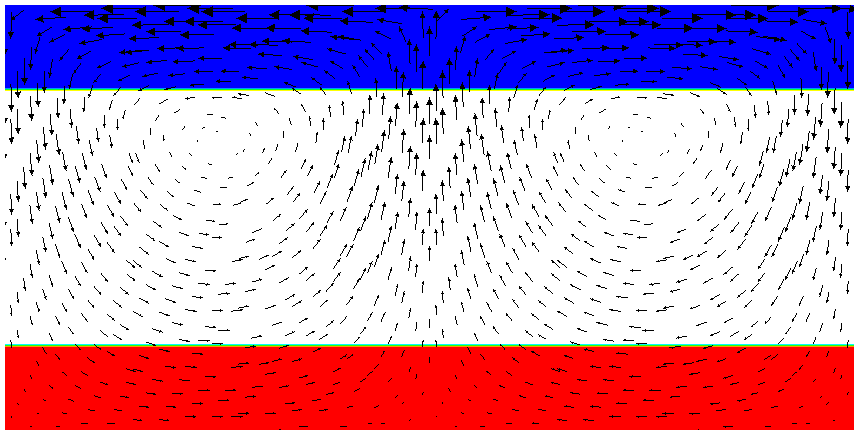
\includegraphics[width=0.3\textwidth]{cookbooks/composition_passive/doc/visit0007.png}
  \hfill
  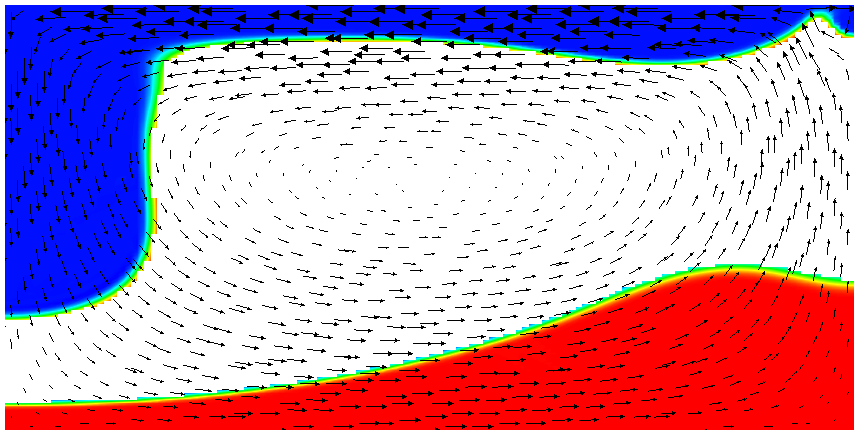
\includegraphics[width=0.3\textwidth]{cookbooks/composition_passive/doc/visit0008.png}
  \hfill
  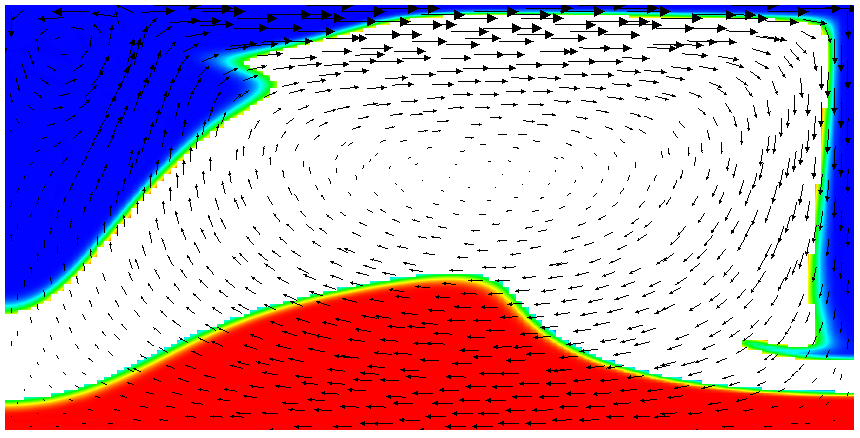
\includegraphics[width=0.3\textwidth]{cookbooks/composition_passive/doc/visit0009.png}
  \\
  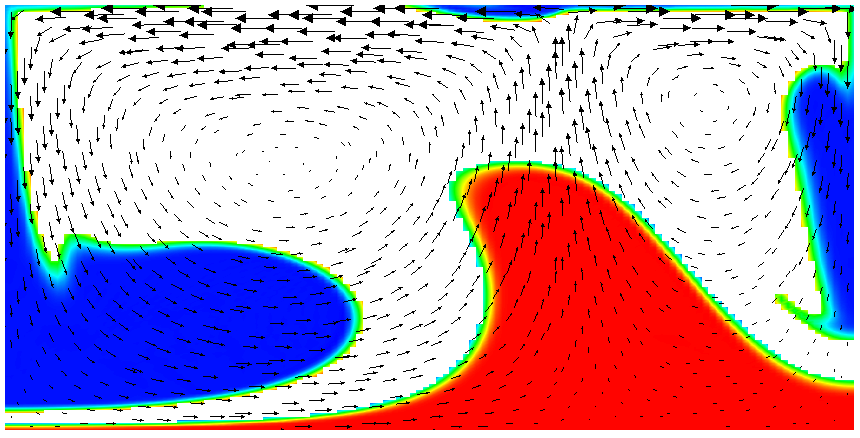
\includegraphics[width=0.3\textwidth]{cookbooks/composition_passive/doc/visit0010.png}
  \hfill
  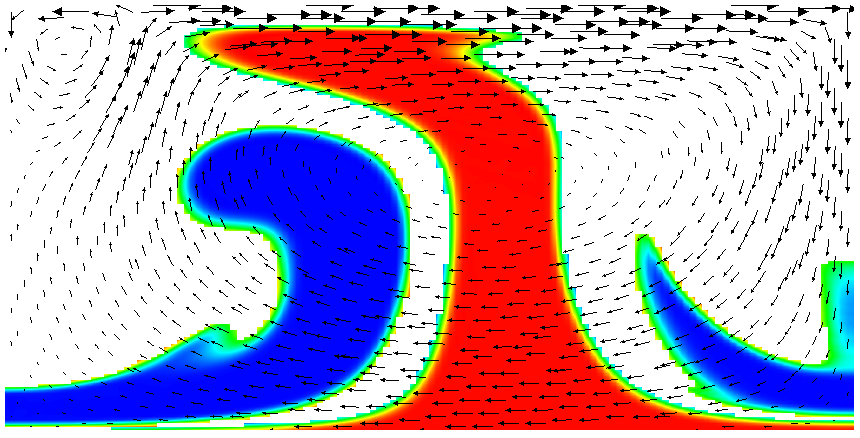
\includegraphics[width=0.3\textwidth]{cookbooks/composition_passive/doc/visit0012.png}
  \hfill
  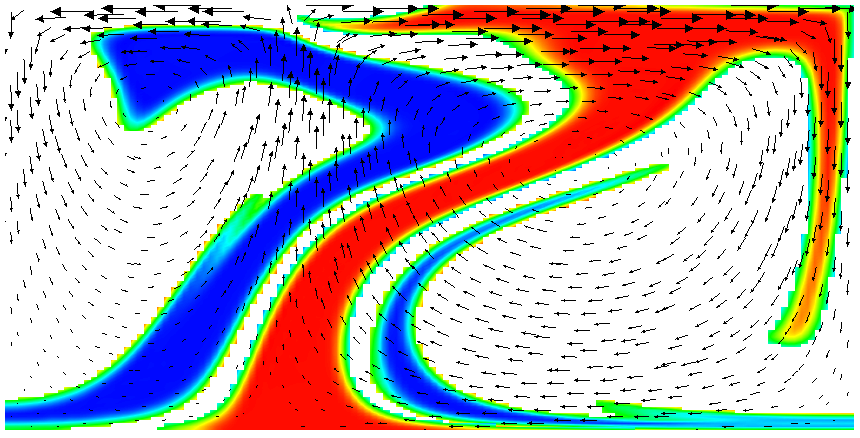
\includegraphics[width=0.3\textwidth]{cookbooks/composition_passive/doc/visit0014.png}
  \caption{\it Passive compositional fields: The figures show, at
    different times in the simulation, the velocity field along with
    those locations where the first compositional field is larger than
    0.5 (in red, indicating the locations where material from the bottom
    of the domain has gone) as well as where the second compositional
    field is larger than 0.5 (in blue, indicating material from the top
    of the domain. The results were obtained with two more global
    refinement steps compared to the
    \url{cookbooks/composition_passive/composition_passive.prm} input file.}
  \label{fig:compositional-passive}
\end{figure}

\begin{figure}
  \centering
  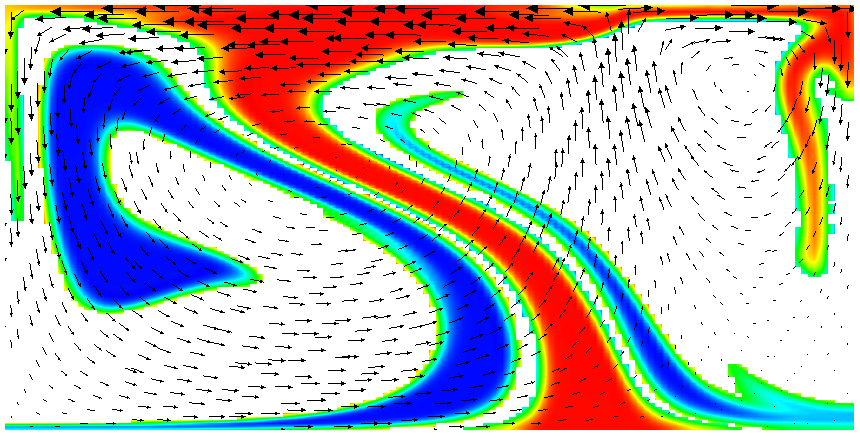
\includegraphics[height=0.3\textwidth]{cookbooks/composition_passive/doc/visit0015.png}
  \hfill
  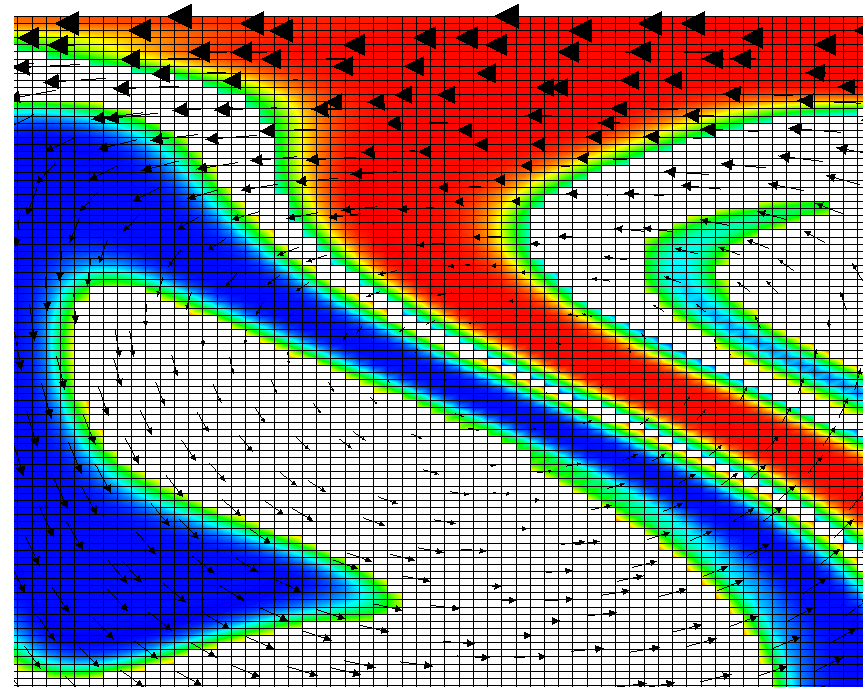
\includegraphics[height=0.3\textwidth]{cookbooks/composition_passive/doc/visit0017.png}
  \caption{\it Passive compositional fields: A later image of the simulation
    corresponding to the sequence shown in
    Fig.~\ref{fig:compositional-passive} (left) and zoom-in on the
    center, also showing the mesh (right).}
  \label{fig:compositional-passive-zoom}
\end{figure}


Fig.~\ref{fig:compositional-passive} shows one aspect of compositional
fields that occasionally makes them difficult to use for very long
time computations. The simulation shown here runs for 20 time units,
where every cycle of the spreading center at the top moving left and
right takes 4 time units, for a total of 5 such cycles. While this is
certainly no short-term simulation, it is obviously visible in the
figure that the interface between the materials has diffused over
time. Fig.~\ref{fig:compositional-passive-zoom} shows a zoom into the
center of the domain at the final time of the simulation. The
figure only shows values that are larger than 0.5, and it looks like
the transition from red or blue to the edge of the shown region is no
wider than 3 cells. This means that the computation is not overly
diffusive but it is nevertheless true that this method has difficulty
following long and thin filaments.%
\footnote{We note that this is no different for particles where the
  position of particles has to be integrated over time and is subject to
  numerical error. In simulations, their location is therefore not the
  exact one but also subject to a diffusive process resulting from
  numerical inaccuracies. Furthermore, in long thin filaments, the
  number of particles per cell often becomes too small and new particles
  have to be inserted; their properties are then interpolated from the
  surrounding particles, a process that also incurs a smoothing penalty.}
This is an area in which \aspect{} may see improvements in the future.


\begin{figure}
  \centering
  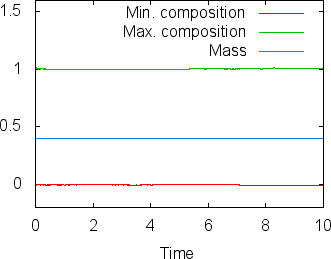
\includegraphics[width=0.4\textwidth]{cookbooks/composition_passive/doc/mass-composition-1.png}
  \caption{\it Passive compositional fields: Minimum and maximum of the first
  compositional variable over time, as well as the mass $m_1(t)=\int_\Omega c_1(\mathbf x,t)$ stored in this variable.}
  \label{fig:compositional-passive-mass}
\end{figure}

A different way of looking at the quality of compositional fields as opposed to
particles is to ask whether they conserve mass. In the current context, the
mass contained in the $i$th compositional field is $m_i(t)=\int_\Omega c_i(\mathbf x,t)$.
This can easily be achieve in the following way, by adding the \texttt{composition statistics}
postprocessor:

\lstinputlisting[language=prmfile]{cookbooks/composition_passive/doc/postprocess.part.prm.out}

While the scheme we use to advect the compositional fields is not strictly
conservative, it is almost perfectly so in practice. For example, in
the computations shown in this section (using two additional global mesh
refinements over the settings in the parameter file
\url{cookbooks/composition_passive/composition_passive.prm}), Fig.~\ref{fig:compositional-passive-mass}
shows the maximal and minimal values of the first compositional fields over time,
along with the mass $m_1(t)$ (these are all tabulated in columns of the
statistics file, see Sections~\ref{sec:running-overview} and \ref{sec:viz-stat}). While
the maximum and minimum fluctuate slightly due to the instability of the finite element
method in resolving discontinuous functions,
the mass appears stable at a value of 0.403646 (the exact value, namely the
area that was initially filled by each material, is 0.4; the difference is a
result of the fact that we can't exactly represent the step function on our
mesh with the finite element space). In fact, the maximal difference in this
value between time steps 1 and 500 is only $\num{1.1e-6}$. In other words,
these numbers show that the compositional field approach is almost exactly mass conservative.
